\documentclass[12pt, a4paper]{article}
\usepackage{meu}
\usepackage{float}

\begin{document}
\capa
\tableofcontents
\cleardoublepage
\listoffigures
\cleardoublepage
\listoftables
\cleardoublepage



\section{Introdução}

O termo \textit{Internet of Things (IoT)}, do português \textit{Internet das Coisas} foi proposto pelo professor britânico, Kevin Ashton do Instituto de Tecnologias de Massachusetts (MIT), no ano de 1999\cite{5} e diz a respeito da forma geral de uma rede que conecta diversos dispositivos, ``coisas'', à internet, através de software, com o objetivo de realizar troca informações\cite{defIot} gerando valor e conhecimento. Dessa forma, um mesmo sistema passava a ser composto por um rede dispersa de dispositivos, como podem ser: sensores, microcontroladores ou eletrodomésticos - como geladeiras, televisores, entre outros.

\subsection*{Camadas dos sistemas envolvendo IoT}\label{Camadas dos sistemas de IoT}

A estrutura geral dos sistemas envolvendo a \textit{Internet das Coisas}, como proposto por Ashton pode ser dividida em três camadas principais\cite{5} que caraterizam as diferentes responsabilidades do sistema:

  \begin{itemize}
      \item Em primeiro lugar, a \textbf{Camada de Percepção}, responsável pela captação dos dados do meio, envolve os sensores e o hardware necessários para a obtém-são da informações relevantes a respeito de fenômenos dispersos e de diferentes naturezas. Exemplos de fenômenos de interesse para os sistemas de IoT são os eventos meteorológicos, biológicos ou físicos como, a temperatura e umidade do solo\cite{3}, do ar\cite{9}, índice de área foliar\cite{8}, quantidade de gás SO$_{2}$\cite{13}, PH do solo\cite{13} entre muitos outros, dependendo do tipo de aplicação que tem por objetivo o sistema.
      \item Em segundo lugar, a \textbf{Camada de Comunicação}, é a responsável pela transmissão dos dados oriundos dos diversos dispositivos conectados com outras camadas, como são: os sensores da camada de percepção, os servidores responsáveis por fazer a análise dos dados, as aplicações encarregadas de disponibilizar a inteligência obtida a partir dos dados, ou ainda outros dispositivos que atuarão em dependência dos valores recebidos. Nesse sentido, é na junção da Camada de Comunicação e a Camada de Percepção que acabam por caraterizar um sistema como sendo de IoT.
      \item Em terceiro lugar, e finalmente, a \textbf{Camada de Aplicação} é a encarregada de dar sentido aos dados coletados pelos sensores, pois é nesse momento que ocorre a apresentação dos mesmos de forma a gerar valor para os usuários do sistema. Dessa forma, uma área onde tem ocorrido uma ampla implementação dos sistemas IoT é na agricultora. Tal fato fica justificado pela relevância e singularidade dos dados que caraterizam uma plantação, os quais variam rapidamente no tempo e no espaço. Assim, a partir dessa informação pode ser identificado qual é o melhor momento e lugar da fazenda realizar o plantio e colheita das diferentes culturas\cite{1}, ou mesmo em quais lugares da plantação ha doenças\cite{2}.
      \end{itemize}

No contexto dos sistemas de Internet das Coisas, a camada de comunicação é a que maiores desafios oferece para os desenvolvedores de soluções desse tipo de sistemas. Isso se justifica, tendo em vista os requisitos como são: as longas distâncias de transmissão de dados, o uso de dispositivos de baixo custo, busca por baixos consumos de energia, entre outros. Nesse sentido, o protocolo de comunicação MQTT, originalmente conhecido como \textit{MQ Telemetry Transport}, tem se tornado praticamente um estândar entre as soluções de IoT, desde que foi proposto.

\cleardoublepage

\section{História do protocolo MQTT}

O protocolo MQTT começou a ser idealizado e planejado durante a década de 1990\cite{historia_breve_resumo_mqtt}, pelos engenheiros Andy Stanford-Clark da IBM e Arlen Nipper da Cirrus Link/Eurotech\cite{historia_introduction_mqtt}.

Andy e Arlen se estavam trabalhando na conexão de oleodutos via satélite, os quais visto a limitação das conexões e o hardware da época perceberam a necessidade de um protocolo de comunicação que utilizasse pouca largura de banda e pouca energia do dispositivo, tendo isso em mente elicitaram os seguintes requisitos\cite{historia_introduction_mqtt}:

\begin{itemize}
    \item Implementação simples;
    \item Uso de QoS, \textit{Quality of Service} por quem publica a mensagem;
    \item Uso eficiente de largura de banda, baixo \textit{overhead};
    \item Baixo custo energético para envio;
    \item Possibilidade de enviar qualquer tipo de dado;
    \item Possibilidade de manter conexões ativas, prontas para enviar e receber dados;
\end{itemize}

Uma vez projetado, foi implementado sua primeira versão no ano de 1999 e batizado MQTT, \textit{MQ Telemetry Transport}, em referência ao produto da IBM MQ Series, que atua na camada de transporte sendo uma ferramenta importante em arquiteturas orientadas a serviços\cite{historia_ibm_mq}.

Esse protocolo de comunicação foi muito utilizado dentro da IBM em diversas aplicações, produtos e serviços desde sua criação até 2010\cite{historia_introduction_mqtt}. Porém nesse momento da história viu-se a possível utilidade da tecnologia em aplicações IoT, com isso o MQTT deixou de ser \textit{software} proprietário apenas utilizado em sistemas embarcados da IBM, para ser um dos principais protocolos utilizados em internet das coisas, com isso foi lançado o MQTT 3.1 o qual pode ser utilizado sem precisar pagar por \textit{royaltys} ou taxas de propriedade.

Com a abertura do protocolo a IBM fez investimentos para criar um ecossistema colaborativo para incentivar o seu uso, principalmente através da \textit{Eclipse Foundation}, uma corporação sem fins lucrativos que visa impulsionar projetos de software livre e tecnologias abertas\cite{historia_eclipse_f}, que gerência mais de 400 repositórios abertos\footnote{Github da Eclipse Foundation: \url{https://github.com/eclipse}}, muitos deles relacionados ao MQTT, como por exemplo:

\begin{itemize}
    \item\textbf{Bibliotecas Paho}\footnote{Implementação da biblioteca em Python:\url{https://github.com/eclipse/paho.mqtt.python}}: Tendo inicio em 2012/2013 o projeto Paho disponibiliza um conjunto de bibliotecas que implementam clientes MQTT em diversas linguagens de programação, sendo a mais conhecida delas em Python, porém foram escritas versões para C++, C, Rust, Java, Go, JavaScript, Ruby, D\ldots
    \item\textbf{Broker Mosquitto}\footnote{Código fonte do Broker: \url{https://github.com/eclipse/mosquitto}}: Servidor que implementa o protocolo MQTT, também chamado de Broker. Por ser \textit{open source} possuí diversos \textit{forks} e customizações, bem como bibliotecas para facilitar seu uso e configuração.
    \item\textbf{Visualizador de dados Streamsheet}\footnote{Github do projeto: \url{https://github.com/eclipse/streamsheets}}: Aplicação JavaScript que permite obter os dados vindos de dispositivos que se comunicam com MQTT, uma plataforma na qual não é necessário escrever código, basta realizar ações de maneira gráfica.
\end{itemize}

Além da implementação dos projetos supracitados a IBM também trabalhou por padronização no protocolo, em 2013 foi anunciado que o MQTT seria padronizado pela OASIS\cite{historia_introduction_mqtt}, empresa sem fins lucrativos que visa padronizar projetos abertos com aprovação de regras de políticas internacionais\cite{historia_oasis}.

Após mais de um ano no dia 29 de outubro de 2014 o MQTT foi aprovado como padrão pela OASIS na sua versão 3.1.1, onde foram adicionados novos requisitos como clientes anônimos, mais códigos de erro ao se inscrever em determinado tópico entre outros.

De 2014 até hoje o MQTT passou por diversas atualizações e melhorias, sendo 5.0 a última versão ratificada pela OASIS em março de 2019\cite{historia_introduction_mqtt}, especificando requisitos necessários para dispositivos IoT modernos, como tratamento de erros e interação com plataformas em nuvem\cite{historia_introduction_mqtt}.

evolução histórica da tecnologia

\cleardoublepage

\section{Aplicações}
    O protocolo MQTT é utilizado em diversas aplicações IoT em várias escalas incluindo a escala industrial. Entre os usos industriais há grandes projetos nas áreas automotivas, logísticas, indústrias, monitoramentos com Smart Home, petrolíferas e aplicações eletrodomésticas.
    \cite{MQTT_Use_Cases}
    
    São exemplos de aplicações consolidadas no mercado: Serviço de compartilhamento de carros da BMW (BMW Mobility Services) e Transporte de amostras entre hospitais e laboratórios utilizando drones autônomos da Matternet.
    \cite{MQTT_Use_Cases}
    
    Ambas as aplicações escolhidas utilizam o protocolo MQTT por meio de uma plataforma chamada HiveMQ, essa plataforma fornece ao usuário um broker MQTT e uma plataforma de mensagem para facilitar o envio e recebimento dos dados de dispositivos IoT, fornecendo dashboards como forma de monitoramento dos dados que passam entre o broker e os clientes conectados com a aplicação.
    \cite{MQTT_Use_Cases, HiveMQ}
    
    \subsection{BMW Mobility Services}\label{BMW Mobility Services}
    
    \begin{figure}[h!]
        \centering
        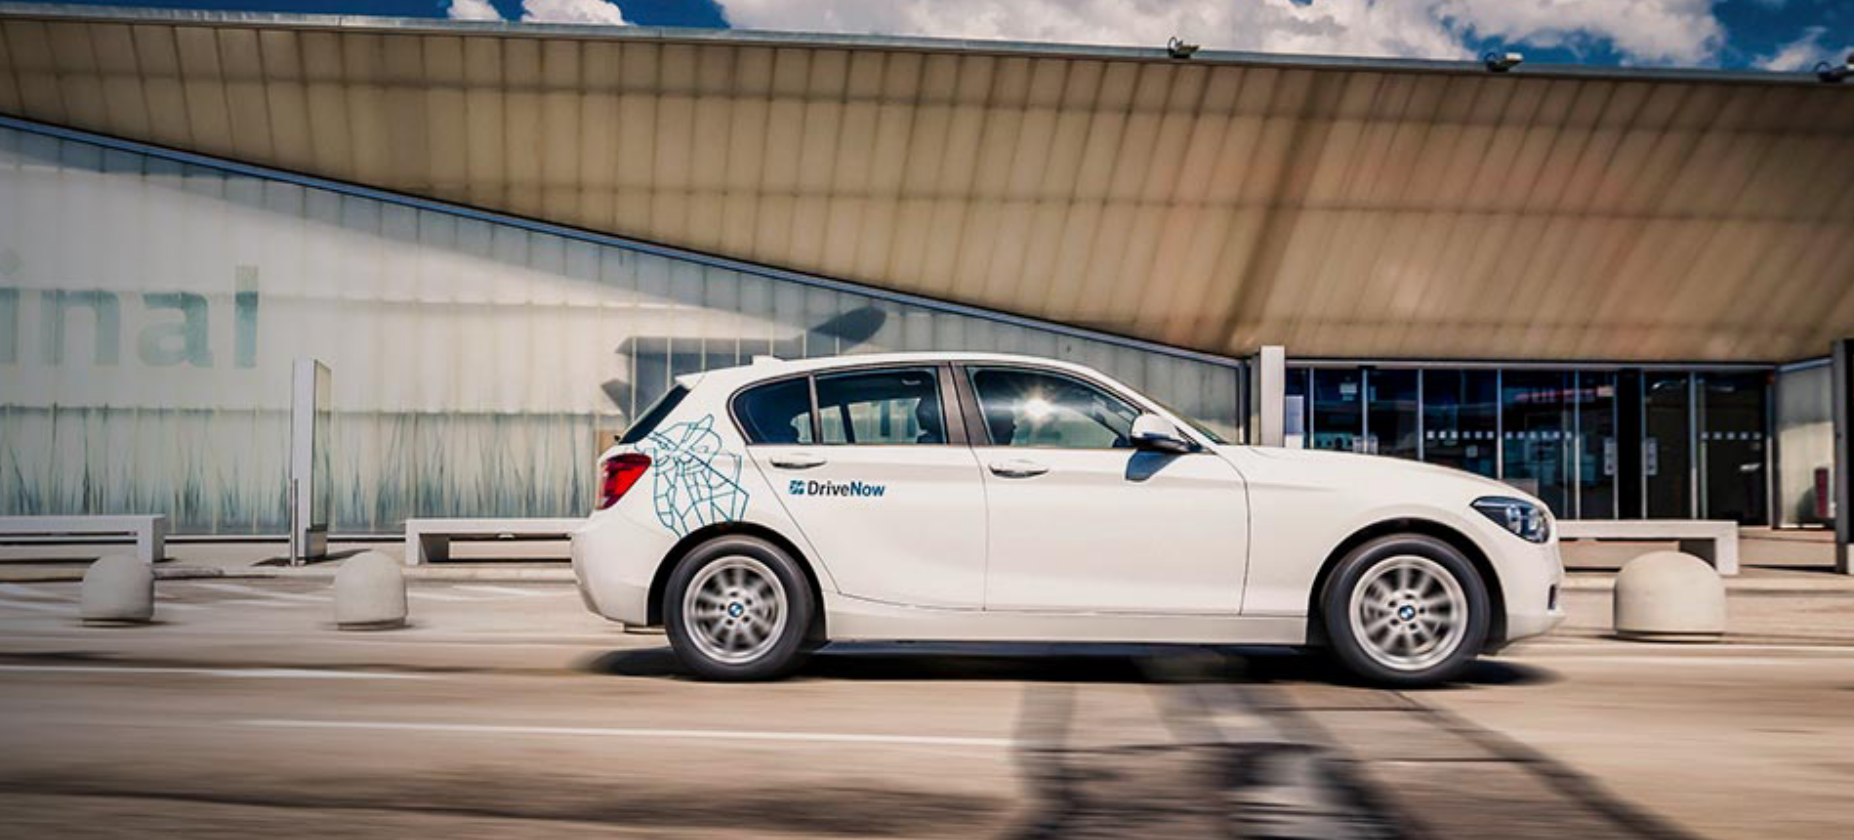
\includegraphics[width=0.8\textwidth]{images/header-cs-bmw-1600.jpg}
        \caption{BMW Mobility Services.}
        \label{fig:BMW_Mobility_Services}
    \end{figure}
    
        A BMW Mobility Services é um grupo empresarial interno ao grupo BMW que desenvolve soluções de mobilidade para população urbana. Entre as soluções de mobilidade desenvolvidas está o serviço de compartilhamento de veículos para operadores de frota. Com esse serviço os operadores de frota podem realizar diversas tarefas de maneira remota, como abrir ou fechar os veículos e obter dados de navegação de cada um. 
        \cite{HiveMQBMW}
        
        Utilizando esse desenvolvimento o grupo BMW lançou um serviço chamado DriveNow que está presente em 12 cidades na Europa.
        \cite{HiveMQBMW}
        
        O uso da HiveMQ foi incluído na plataforma de mensagens do compartilhamento de veículos em 2014. Em razão do sucesso do uso do protocolo MQTT e da plataforma foi realizada a extensão do uso de ambos para mensagens internas que enviam dados entre microsserviços de backend da BMW Mobility Services.  
        \cite{HiveMQBMW}
        
    \subsection{Matternet Autonomous Drones}\label{Matternet Autonomous Drones}
    
    \begin{figure}[h!]
        \centering
        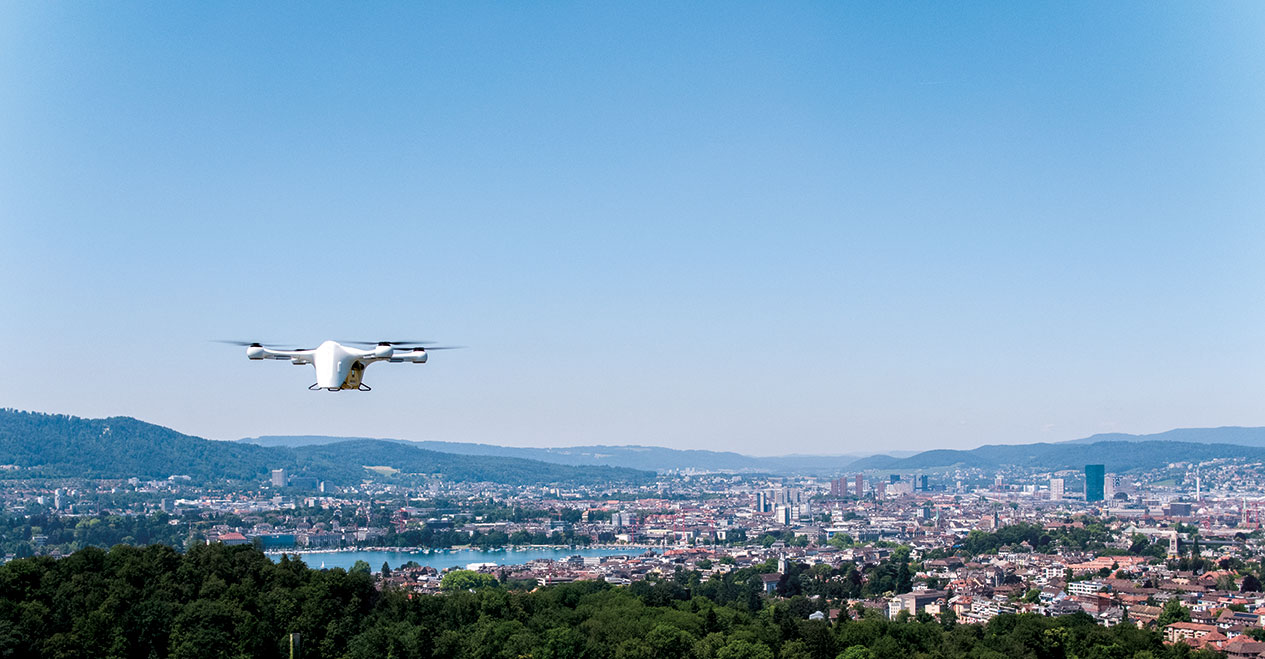
\includegraphics[width=0.8\textwidth]{images/matternet-zurich.jpg}
        \caption{Matternet Autonomous Drones.}
        \label{fig:Matternet_Autonomous_Drones}
    \end{figure}
    
        A Matternet é uma startup, localizada na Califórnia, que utiliza drones autônomos para transporte de amostras entre hospitais e laboratórios. Essa forma de transporte se mostra consideravelmente mais eficiente que as formas convencionais (carros, ônibus ou motos) pois o tempo relativo à entrega é reduzido em razão da eliminação de fatores como congestionamentos e desvios na rota. Com os drones é possível realizar voos que seguem uma rota direta para o destino, diminuindo assim a distância percorrida.
        \cite{HiveMQDrone}
        
        Em razão dos drones realizarem os voos de forma autônoma não é necessário que um piloto realize as funções, porém órgãos reguladores locais de Zurich exigem que um operador humano tenha acesso em tempo real a dados do drone como posição, além de conseguir realizar o controle pilotando-o se for necessário em intercorrências. Além da preocupação governamental relacionada ao modo de voo também é necessário que os voos sejam sincronizados com o espaço aéreo de outras aeronaves, pois os drones podem realizar voos em regiões de hospitais em que há helipontos.
        \cite{HiveMQDrone}
        
        Para que o projeto fosse executado foi necessária a montagem de um esquema com drones autônomos, estações de pouso e uma plataforma logística baseada em nuvem. Essa plataforma logística utiliza o protocolo MQTT juntamente com HiveMQ para comunicação em tempo real dos voos. Os drones enviam mensagens MQTT para o broker da HiveMQ da plataforma logística, como o protocolo suporta comunicação bidirecional é possível realizar a leitura dos dados e controle dos drones caso necessário juntamente com controle do tráfico aéreo.
        \cite{HiveMQDrone}

\cleardoublepage

\section{Embasamento teórico}

\subsection{Terminologia}\label{Terminologia}

Para um melhor entendimento do protocolo de comunicação MQTT é necessário entender a terminologia própria utilizada pelo protocolo. Dessa forma, alguns dos termos de interesse são:

\begin{itemize}
    \item \textbf{Conexão de rede}: se refere ao serviço provido pelo protocolo de comunicação na camada subjacente (TCP/IP) ao protocolo MQTT, e que permite o envio de informação entre os dispositivos.
    \item \textbf{Mensagem}: representa a informação que se deseja transmitir e que portanto constitui o objetivo da comunicação. De forma geral, e pelas caraterísticas do protocolo, a mensagem deve ocupar o mínimo espaço possível - na maioria dos casos é um único valor.
    \item \textbf{Cliente}: programa ou dispositivo que irá enviar ou receber informação. Nesse sentido o cliente deve ser capaz de:
    \begin{itemize}
        \item iniciar uma conexão com o servidor,
        \item realizar a publicação de informações em tópicos,
        \item realizar a subscrição a tópicos de interesse,
        \item realizar o cancelamento de uma subscrição e,
        \item finalizar uma conexão com o servidor.
    \end{itemize}
    \item \textbf{Broker}: programa ou serviço que intermediá e gerência a informação, o envio e recebimento de dados dos clientes, é comum se referir ao mesmo como servidor. Nesse sentido o servidor deve ser capaz de:
    \begin{itemize}
        \item gerencia as conexões como os clientes,
        \item gerenciar as mensagens publicadas pelos clientes,
        \item gerenciar as subscrições dos clientes e,
        \item retransmitir as mensagens recebidas aos clientes.
    \end{itemize}
    \item \textbf{Sessão}: se corresponde com o período de interação entre um cliente e um servidos, durante o qual é mantido um grupo de informações que representam o estado da comunicação, podendo ser composto por mais de uma conexão.
    \item \textbf{Subscrição}: é o ato de que o cliente desempenha para indicar ao servidor interesse em receber atualizações sobre a mudança de um tópico. Dessa forma, uma subscrição se encontra composta por um Filtro de Tópicos, para um ou mais tópicos, e um valor indicando a Qualidade de Serviço deseja (QoS).
    \item \textbf{Subscrição compartilhadas}: são subscrições que se encontram associadas com mais de uma sessão de comunicação entre o cliente e o servidor. Dessa forma, permitem um maior rango de padrões de comunicação.
    \item \textbf{Caracteres mágicos}: também chamados de Wildcards, permitem ao cliente indicar interesse em receber notificações de mais um tópico, para isso fazendo uso de caracteres que definem o padrão dos tópicos desejados.
    \item \textbf{Nome de Tópico}: rótulo ou identificador de uma informação específica dentro do broker e que é constantemente atualizada pelos cliente quando publicam uma nova informação no tópico.
    \item \textbf{Filtro de Tópico}: é uma expressão contida numa subscrição é que se corresponde com um ou mais tópicos
    \item \textbf{Paquete MQTT}: conjunto de informação útil à comunicação cliente-servidor envida através da conexão de rede. O protocolo MQTT especifica 15 tipos de pacotes diferentes, os quais serão especificados a continuação.
\end{itemize}

\cleardoublepage

\section{Características técnicas}
\subsection{Formato dos pacotes MQTT}\label{Formato dos pacotes MQTT}

O envio de dados através do protocolo MQTT utiliza diferentes tipos de pacotes, cada um deles contendo obrigatoriamente um cabeçalho de tamanho fixo, o qual pode ser complementado por um segundo cabeçalho de tamanho variável e um bloco de carga útil, ambos opcionais.

\begin{table}[h!]\caption{Estrutura básica comum a todos os pacotes MQTT.}
\centering
\begin{tabular}{|l|}
\hline
\textbf{Cabeçalho fixo}     \\ \hline
\textbf{Cabeçalho variável} \\ \hline
\textbf{Carga útil}         \\ \hline
\end{tabular}
\end{table}

\textbf{Cabeçalho fixo}

Dentro do protocolo MQTT é no cabeçalho fixo onde é especificado o tipo de pacote que esta sendo enviado, e portanto a sua função no processo de comunicação.

\begin{table}[htb!]\caption{Estrutura do cabeçalho fixo utilizado no protocolo MQTT.}
\centering
\resizebox{\textwidth}{!}{%
\begin{tabular}{|c|cccccccc|}
\hline
\textbf{Bit} &
  \multicolumn{1}{m{.08\textwidth}|}{\textbf{7}} &
  \multicolumn{1}{m{.08\textwidth}|}{\textbf{6}} &
  \multicolumn{1}{m{.08\textwidth}|}{\textbf{5}} &
  \multicolumn{1}{m{.08\textwidth}|}{\textbf{4}} &
  \multicolumn{1}{m{.08\textwidth}|}{\textbf{3}} &
  \multicolumn{1}{m{.08\textwidth}|}{\textbf{2}} &
  \multicolumn{1}{m{.08\textwidth}|}{\textbf{1}} &
  \multicolumn{1}{m{.08\textwidth}|}{\textbf{0}} \\ \hline
  %\textbf{0} \\ \hline
\textbf{Byte 1} & \multicolumn{4}{c|}{\textbf{Tipo de pacote MQTT}} & \multicolumn{4}{c|}{\textbf{Sinais específicos do pacote}} \\ \hline
\textbf{Byte 2} & \multicolumn{8}{c|}{\multirow{2}{*}{\textbf{Espaço restante}}}                                                 \\ \cline{1-1}
\textbf{. . .}  & \multicolumn{8}{c|}{}                                                                                          \\ \hline
\end{tabular}%
}
\end{table}

\cleardoublepage

\textbf{Tipo de pacote MQTT}

Se encontra especificado nos 4 bits mais significativos do primeiro byte da cabeçalho fixo, os quais codificam um número inteiro entre 0 e 15, que por sua vez representa o tipo de pacote, como relacionado na tabela a continuação.

\begin{table}[!htb]\caption{Tipos de pacotes utilizados pelo protocolo MQTT.}
\centering
\resizebox{\textwidth}{!}{%
\begin{tabular}{|l|l|l|l|}
\hline
\multicolumn{1}{|c|}{Tipo} & \multicolumn{1}{c|}{Código} & \multicolumn{1}{c|}{Remetente} & \multicolumn{1}{c|}{Descrição} \\ \hline
Reserved    & 0  & -        & Reservado                                \\ \hline
CONNECT     & 1  & Cliente  & Solicitação 				de conexão               \\ \hline
CONNACK     & 2  & Servidor & Confirmação de conexão                   \\ \hline
PUBLISH     & 3  & Ambos    & Publicar mensagem                        \\ \hline
PUBACK      & 4  & Ambos    & Publicar confirmação (QoS 1)             \\ \hline
PUBREC      & 5  & Ambos    & Publicar recebimento (QoS 2 – parte 1)   \\ \hline
PUBREL      & 6  & Ambos    & Publicar lançamento (QoS 2 – parte 2)    \\ \hline
PUBCOMP     & 7  & Ambos    & Publicar conclusão (QoS 2 – parte 3)     \\ \hline
SUBSCRIBE   & 8  & Cliente  & Solicitação de inscrição                 \\ \hline
SUBACK      & 9  & Servidor & Confirmação de inscrição                 \\ \hline
UNSUBSCRIBE & 10 & Cliente  & Solicitação de cancelamento de inscrição \\ \hline
UNSUBACK    & 11 & Servidor & Confirmação de cancelamento de inscrição \\ \hline
PINGREQ     & 12 & Cliente  & Solicitação de PING                      \\ \hline
PINGRESP    & 13 & Servidor & Resposta de PING                         \\ \hline
DISCONNECT  & 14 & Ambos    & Notificação de desconexão                \\ \hline
AUTH        & 15 & Ambos    & Troca de autenticação                    \\ \hline
\end{tabular}
}
\end{table}

\textbf{Sinais específicos do pacote}

Complementa a informação do tipo do pacote, e se encontra representado pelos 4 bits menos significativos do primeiro byte. Dessa forma, indica diferentes modos em que pode ser usado o mesmo formato de pacote.

\textbf{Espaço restante}

Informação útil e de controle dependentes de cada tipo de pacote.

\cleardoublepage

\subsection{Função dos pacotes MQTT}

\begin{itemize}
    \item \textbf{CONNECT (Requisição de Conexão)}: é o primeiro pacote que deve ser enviado pelo cliente no momento após ter estabelecido um conexão de rede com servidor. Entre as informações enviadas se encontra um identificador único para o cliente, entre outras informações opcionais como usuário e senha.
    \item \textbf{CONNACK (Reconhecimento de conexão)}: é o pacote enviado pelo servidor em resposta ao recebimento do pacote CONNECT enviado pelo cliente, e que deve ser recebido antes do pacote AUTH. Em caso do cliente não receber um pacote do tipo CONNACK em um tempo razoável o mesmo deve encerar a conexão com o servidor e tentar novamente.
    \item \textbf{PUBLISH (Publicar mensagem)}: são os pacotes encarregados de carregar as mensagens entre o servidor e os clientes podendo ir em ambas as direções.
    \item \textbf{PUBACK (Reconhecimento de publicação)}: é o pacote enviado em resposta a um PUBLISH realizado com QoS 1.
    \item \textbf{PUBREC (Recebimento de publicação)}: é o pacote enviado em resposta a um PUBLISH representa a segunda parte do intercambio de mensagens realizado com QoS 2.
    \item \textbf{PUBREL (Liberação de publicação)}: é o pacote enviado em resposta a um PUBREC e representa a terceira parte do intercambio de mensagens realizado com QoS 2.
    \item \textbf{PUBCOMP (Publicação completada)}: é o pacote enviado em resposta a um PUBREL e representa a quarta e última parte do intercambio de mensagens realizado com QoS 2.
    \item \textbf{SUBSCRIBE (Requisição de subscrição)}: é o pacote enviado pelo cliente ao servidor como solicitude para a criação de uma ou mais assinaturas, registrando o interesse em receber informação de um ou mais tópicos, junto com o tipo de qualidade do serviço máxima (QoS) desejada com a qual o servidor pode enviar uma mensagem ao cliente.
    \item \textbf{SUBACK (Reconhecimento de subscrição)}: é o pacote enviado pelo servidor ao cliente com o objetivo de confirmar o recebimento e processamento de um pacote do tipo SUBSCRIBE. Entre as informações contidas pelo pacote tem uma lista indicando a qualidade do serviço concedida ao cliente para cada tópico e em caso de ter sido negada a subscrição é enviado um sinal justificando o motivo do mesmo.
    \item \textbf{UNSUBSCRIBE (Requisição de cancelamento de subscrição)}: é o pacote utilizado pelo cliente para indicar que já não deseja receber atualizações da mudança de valore de um tópico.
    \item \textbf{UNSUBACK (Reconhecimento de cancelamento de subscrição)}: é o pacote enviado pelo servidor ao cliente indicando conhecimento do pedido de anulação de subscrição iniciado pelo pacote de UNSUBSCRIBE.
    \item \textbf{PINGREQ (Requisição de PING)}: é o pacote envido pelo cliente ao servidor, é pode ser utilizado para: indicar ao servido que o cliente se encontra ativo e à espera de qualquer pacote MQTT, requerer ao servidor que responda se se encontra ativo, ou, ainda, para verificar se a conexão à rede se encontra em funcionamento.
    \item \textbf{PINGRESP (Resposta a uma Requizição de PING)}: é a resposta enviada pelo servidor quando recebe uma mensagem do tipo PINGREQ, sinalizando que o mesmo se encontra em funcionamento.
    \item \textbf{DISCONNECT (Requisição de desconexão)}: é o pacote de controle final enviado pelo cliente ao servidor, indicando a intenção e o motivo pelo qual a conexão de rede está sendo fechada.
    \item \textbf{AUTH (Intercambio de autentificações)}: é pacote enviado para a troco de informação referente a autentificação de informação, servindo dessa forma para a prevenção de erros de comunicação.
\end{itemize}

\cleardoublepage

\section{Segurança}
    O desenvolvimento rápido de dispositivos IoT e o grande crescimento desse ramo da tecnologia no mercado se deu muitas vezes em detrimento da consideração de segurança e limitações dos dispositivos. Esse aspecto, juntamente com o fato desse alto número de dispositivos se conectar à Internet e ter capacidade de armazenar diversas informações dos usuários traz grande risco a ataques. 
    \cite{MQTT_Vunerabilities}
    
    Como exemplo de ataque à dispositivos inteligentes há o ataque à empresa Dyn DNS. A empresa sofreu um ataque de negação de serviço distribuído (Distributed Denial of Service – DDoS) orquestrado por uma botnet. Nesse ataque o malware atingiu diversos dispositivos por meio de um ataque de força bruta em que realizava o acesso à interface do dispositivo e realizava upload de seu código. Esse DDoS conseguiu gerar um fluxo de pacotes TCP e UDP e atacar uma porta com sucesso. Esse ataque e vários outros demonstram a importância da segurança em dispositivos IoT.
    \cite{MQTT_Vunerabilities, DDoS}
    
    Os DDoS estão entre os tipos mais comuns de ataques na Internet em que há uma tentativa maliciosa de interromper o tráfego de servidores, serviços ou rede por meio da sobrecarga no destino com enxurradas de tráfego. A botnet é um grupo de dispositivos infectados com malware que passa a realizar o ataque, quando é estabelecida a botnet o invasor direciona instruções para cada dispositivo infectado. Assim um endereço de IP pode receber solicitações de diversos dispositivos controlados pelo malware ao ponto de extrapolar a capacidade do servidor. Como cada robô (bot) é um dispositivo de Internet legítimo não é uma tarefa fácil para o servidor ou rede de destino separar os dispositivos que realizam os ataques de dispositivos inocentes.
    \cite{DDoS, Botnet}
    
    O protocolo MQTT possui suporte para diferentes mecanismos de segurança, porém a maior parte deles não é configurada como padrão como criptografia de dados e autenticação de entidades. Cada cliente MQTT possui um ID único de cliente e, se houver tentativa de conexão com um ID já conectado, a primeira conexão é encerrada. Os mecanismos de autenticação que usam o endereço de controle de acesso ao meio (MAC – Media Acess Control) são controlados pelos brokers que registram essa informação dos dispositivos quando há tentativa de conexão. A autorização de acesso pode ser realizada utilizando mecanismos de lista de controle de acesso (ACL – Acess Control Lists), que promove um meio de proteção de informações em que é possível restringir o acesso a diferentes porções de diretórios ou entradas para estes diretórios.
    \cite{MQTT_Vunerabilities, Acess_Control_Lists}
    
    A confiabilidade também é um aspecto importante para sistemas seguros e pode ser tratada na camada de aplicação com a realização da criptografia da mensagem a ser publicada. Essa criptografia pode ser implementada ponta a ponta ou cliente a broker. Na criptografia cliente-broker o broker realiza a descriptografia da informação que está sendo publicada e criptografa valores que serão enviados a outros clientes. Na cripotrafia ponto a ponto o broker não descriptografa a informação, apenas enviando o texto criptografado a outros dispositivos, utilizando menos recursos computacionais e menos energia por trabalhar apenas como mensageiro. 
    \cite{MQTT_Vunerabilities}
    
    Quanto a camadas mais baixas também há possibilidade de adição de mecanismos de segurança.  Uma forma confiável de garantir a segurança de canais de comunicação na camada de transporte é utilizar o protocolo Transport Layer Security (TLS) para Transmission Control Protocol (TCP), que permite que duas partes identifiquem e autentiquem uma a outra por meio de certificados digitais e realizem comunicação com confidencialidade e integridade de dados. No caso do uso de User Datagram Protocol (UDP) uma forma de garantir a segurança é o uso de Datagram Transport Layer Security (DTLS) que é baseado no protocolo TLS e fornece garantias de segurança da mesma forma que o TLS.
    \cite{TLS, TLS2, DTLS}
    
    Um desafio relacionado à implantação de bons mecanismos de segurança é a falta de recursos pois, tomando como exemplo a implementação do protocolo TLS em que o overhead gerado pode ser muito grande para dipositivos pequenos e com recursos limitados. Outros dispositivos IoT podem nem oferecer suporte a esse protocolo.
    \cite{MQTT_Vunerabilities}
    
    Podem ser utilizados diversos algoritmos como Advanced Encryption Standard (AES) como algoritmos de criptografia, sendo o AES o mais utilizado. 
    \cite{MQTT_DOC}
    
    Dentre as formas de aumentar a segurança com o protocolo MQTT estão: autenticação e autorização de clientes pelo servidor, autenticação do servidor pelos clientes, verificação da integridade dos dados por meio de valores de hash, uso de VPN, realizar a detecção de comportamentos anormais como muitas tentativas de conexão, entre outros.
    \cite{MQTT_DOC}
    
    Outra forma de aumentar a segurança é o uso do protocolo Secure MQTT, nas quais a implementação do servidor oferece TLS e utilizam a porta 8833. O uso nesse formato possui cadastro na Autoridade para Atribuição de Números da Internet (IANA – Internet Assigned Numbers Authority) como secure-mqtt. A IANA supervisiona a atribuição global dos números na Internet como endereços IP, servidores raiz de DNS e registros de protocolos de comunicação como no caso do MQTT.
    \cite{MQTT_DOC, IANA}

\cleardoublepage

\section{Exemplo Prático}

\subsection{Descrição da aplicação implementada}

A modo de exemplo é apresentada uma aplicação que a partir de um ESP32 realiza a leitura da temperatura do ambiente fazendo uso de um sensor BMP280 e envia ela como um tópico para um broker que se encontra conectado na mesma rede e que por sua vez tem a capacidade de alterar o estado de um LED conectado ao ESP32.

\subsection{Descrição das tecnologias e dispositivos utilizados}

Para implementar a aplicação apresentada foram utilizados os seguintes componentes e tecnologias:

\begin{itemize}
    \item Esp32:
        \begin{itemize}
            \item Sensor Adafruit BMP-280;
            \item Led embutido no Esp32;
            \item C/C++ (Framework Arduino e ESP-IDF);
        \end{itemize}
    \item Raspberry:
        \begin{itemize}
            \item Docker executando o broker mosquitto;
            \item Cliente inscrito no tópico ``\#''
        \end{itemize}
\end{itemize}

\cleardoublepage

\subsection{Esquema da aplicação utilizada}

Dessa forma, o funcionamento da aplicação implementada se encontra resumido no seguinte esquema:

\begin{figure}[h!]
    \centering
    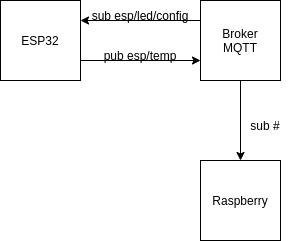
\includegraphics[width=.7\textwidth]{aplication}
    \caption{\label{fig:aplication} Dispositivos e tópicos utilizados}
\end{figure}

\cleardoublepage

\subsection{Métodos principais da aplicação}

\begin{lstlisting}
void setup() {
    if (!sensor.begin(BMP280_ADDRESS)) {
        if(!sensor.begin(BMP280_ADDRESS_ALT)) {
            delay(1000);
            ESP.restart();
        }
    }
    pinMode(LED_PIN, OUTPUT);
    wifiConnect();
    MqttConnect();
    xTaskCreate(taskSendTemperature, "send", 20000, NULL, 1, &handle);
}

void loop() {
    if (!mqttClient.connected()) {
        MqttConnect();
    }
    mqttClient.loop();
}
\end{lstlisting}


\cleardoublepage

\section{Conclusões}

O presente trabalho foi desenvolvido com o intuito de ajudar a esclarecer e apresentar aspectos gerais e principalmente técnicos a respeito do protocolo de comunicação MQTT. Dessa forma, serviu para trazer um melhor entendimento sobre o mesmo, ajudando a esclarecer aspectos como a sua história, caraterísticas principais, contexto de uso, tipos de pacotes utilizados, entre outros. Por outro lado, o presente trabalho foi útil para o desenvolvimento de capacidades necessárias para o trabalho em equipe por partes dos participantes.

\cleardoublepage

\bibliography{ref}

\end{document}
